\documentclass[a4paper,12pt]{article}
\usepackage{graphicx}
\usepackage[UTF8]{ctex}
\usepackage{fontspec}
\usepackage{booktabs}
\usepackage{float}%浮动体
\usepackage{amsmath,amssymb}
\usepackage{fancyhdr}
%\usepackage{xcolor}
\usepackage{colortbl}
\usepackage{geometry}
\geometry{top=2cm,bottom=2cm,left=1cm,right=1cm}
\begin{document}
	\begin{figure}[H]
	\begin{center}
		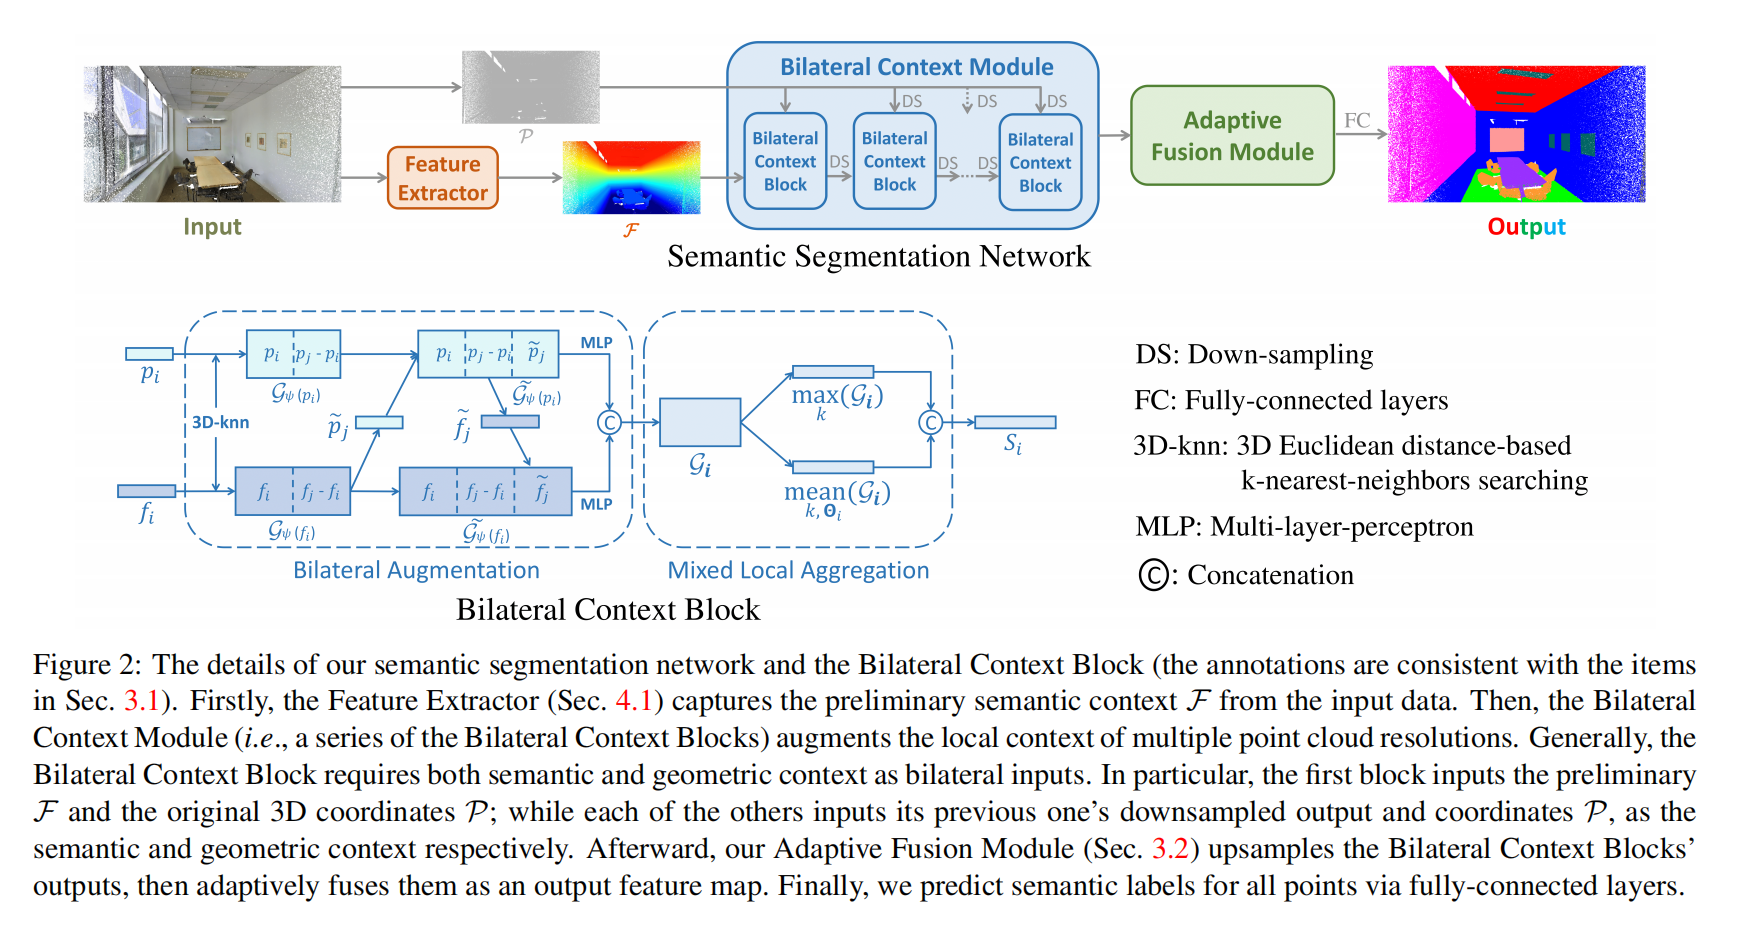
\includegraphics[width=1\textwidth]{img/Bil_Aug_Adap_Fusion.png} 
		\caption{Bil\_Aug\_Adap\_Fusion}
	\end{center}
\end{figure}


\textbf{分析}:
\begin{itemize}
	\item 随机采样,然后通过local spatial encoding, Attentive Pooling通过类似ResNet的结构组织起来,对特征进行聚合。(能够处理较大规模的数据)
	\item 
\end{itemize}
$$
\begin{aligned}
	&\mathcal{G}_{\psi}\left(p_{i}\right)=\left[p_{i} ; p_{j}-p_{i}\right]\\
	&\mathcal{G}_\psi\left(f_{i}\right)=\left[f_{i} ; f_{j}-f_{i}\right]\\
	&\tilde{p}_{j}=M\left(\mathcal{G}_\psi\left(f_{i}\right)\right)+p_{j} . \quad \tilde{p}_{j} \in \mathbb{R}^{3}\\
	&\tilde{\mathcal{G}}_{\psi}\left(p_{i}\right)=\left[p_{i} ; p_{j}-p_{i} ; \tilde{p}_{j}\right]\\
	&\tilde{f}_{j}=M\left(\tilde{\mathcal{G}}_{\psi}\left(p_{i}\right)\right)+f_{j}, \tilde{f}_{j} \in \mathbb{R}^{d}\\
	&\tilde{\mathcal{G}}_{\psi}\left(f_{i}\right)=\left[f_{i} ; f_{j}- f_{i} ; \tilde{f_{j}}\right] .\\
	&\mathcal{G}_{i}=\operatorname{con} \operatorname{cat}\left(M\left(\tilde{\mathcal{G}}_{\varphi}\left(p_{i}\right)\right), M\left(\tilde{\mathcal{G}}_{\psi}\left(f_{i}\right)\right)\right)\\
	&\mathcal{L}\left(p_{i}\right)=|| \frac{1}{k} \sum_{j=1}^{k} \tilde{p_{j}}-\left.p_{i}\right||_{2},保持总体二点集合完整性
\end{aligned}
$$
$$s_{i}=\operatorname{concat}\left(\max _{k}\left(\mathcal{G}_{i}\right), \operatorname{mean}_{k, \Theta_{i}}\left(\mathcal{G}_{i}\right)\right)$$

	\begin{figure}[H]
	\begin{center}
		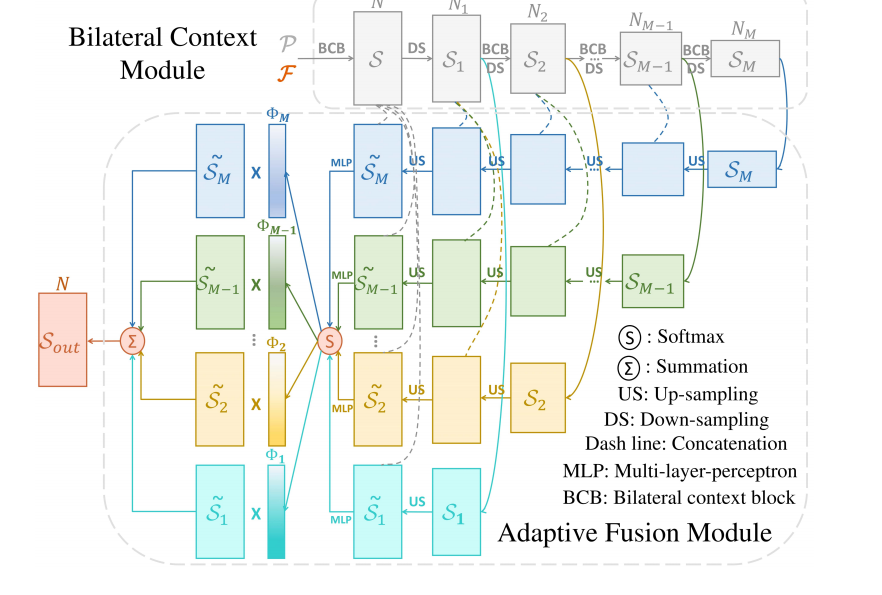
\includegraphics[width=1\textwidth]{img/Adap_Fusion_Mod.png} 
		\caption{Adap\_Fusion\_Mod}
	\end{center}
\end{figure}
\end{document}